% A LaTeX (non-official) template for ISAE projects reports
% Copyright (C) 2014 Damien Roque
% Version: 0.2
% Author: Damien Roque <damien.roque_AT_isae.fr>

\documentclass[oneside,12pt]{book}
\usepackage[utf8]{inputenc}
\usepackage[T1]{fontenc}
\usepackage[frenchb]{babel}
\usepackage{a4wide}
\usepackage{graphicx}
\usepackage{multirow}
\graphicspath{{images/}}
\usepackage{subfig}
\usepackage{tikz}
\usetikzlibrary{shapes,arrows}
\usepackage{pgfplots}




\pgfplotsset{compat=newest}
\pgfplotsset{plot coordinates/math parser=false}
\newlength\figureheight
\newlength\figurewidth
\pgfkeys{/pgf/number format/.cd,
set decimal separator={,\!},
1000 sep={\,},
}
\usepackage{ifthen}
\usepackage{ifpdf}
\usepackage{sectsty}
\sectionfont{\LARGE}
\subsectionfont{\large}
\renewcommand{\thesection}{\arabic{section}}
\usepackage{enumitem}
\usepackage{biblatex}


\ifpdf
\usepackage[pdftex]{hyperref}
\else
\usepackage{hyperref}
\fi
\usepackage{color}
\hypersetup{%
colorlinks=true,
linkcolor=black,
citecolor=black,
urlcolor=black}

\renewcommand{\baselinestretch}{1.05}
\usepackage{fancyhdr}
\renewcommand\headrule{}
\pagestyle{plain}
\fancyfoot{}
\fancyhead[LE,RO]{\bfseries\thepage}
\fancyhead[RE]{\bfseries\nouppercase{\leftmark}}
\fancyhead[LO]{\bfseries\nouppercase{\rightmark}}
\setlength{\headheight}{15pt}
\renewcommand{\headrulewidth}{0pt}

\let\headruleORIG\headrule
\renewcommand{\headrule}{\color{black} \headruleORIG}
\renewcommand{\headrulewidth}{1.0pt}
\usepackage{colortbl}
\arrayrulecolor{black}

\fancypagestyle{plain}{
  \fancyhead{}
  \fancyfoot[C]{\thepage}
  \renewcommand{\headrulewidth}{0pt}
}

\makeatletter
\def\@textbottom{\vskip \z@ \@plus 1pt}
\let\@texttop\relax
\makeatother

\makeatletter
\def\cleardoublepage{\clearpage\if@twoside \ifodd\c@page\else%
  \hbox{}%
  \thispagestyle{empty}%
  \newpage%
  \if@twocolumn\hbox{}\newpage\fi\fi\fi}
\makeatother

\usepackage{amsthm}
\usepackage{amssymb,amsmath,bbm}
\usepackage{array}
\usepackage{bm}
\usepackage{multirow}
\usepackage[footnote]{acronym}

\newcommand*{\SET}[1]  {\ensuremath{\mathbf{#1}}}
\newcommand*{\VEC}[1]  {\ensuremath{\boldsymbol{#1}}}
\newcommand*{\FAM}[1]  {\ensuremath{\boldsymbol{#1}}}
\newcommand*{\MAT}[1]  {\ensuremath{\boldsymbol{#1}}}
\newcommand*{\OP}[1]  {\ensuremath{\mathrm{#1}}}
\newcommand*{\NORM}[1]  {\ensuremath{\left\|#1\right\|}}
\newcommand*{\DPR}[2]  {\ensuremath{\left \langle #1,#2 \right \rangle}}
\newcommand*{\calbf}[1]  {\ensuremath{\boldsymbol{\mathcal{#1}}}}
\newcommand*{\shift}[1]  {\ensuremath{\boldsymbol{#1}}}

\newcommand{\eqdef}{\stackrel{\mathrm{def}}{=}}
\newcommand{\argmax}{\operatornamewithlimits{argmax}}
\newcommand{\argmin}{\operatornamewithlimits{argmin}}
\newcommand{\ud}{\, \mathrm{d}}
\newcommand{\vect}{\text{Vect}}
\newcommand{\sinc}{\ensuremath{\mathrm{sinc}}}
\newcommand{\esp}{\ensuremath{\mathbb{E}}}
\newcommand{\hilbert}{\ensuremath{\mathcal{H}}}
\newcommand{\fourier}{\ensuremath{\mathcal{F}}}
\newcommand{\sgn}{\text{sgn}}
\newcommand{\intTT}{\int_{-T}^{T}}
\newcommand{\intT}{\int_{-\frac{T}{2}}^{\frac{T}{2}}}
\newcommand{\intinf}{\int_{-\infty}^{+\infty}}
\newcommand{\Sh}{\ensuremath{\boldsymbol{S}}}
\newcommand{\C}{\SET{C}}
\newcommand{\R}{\SET{R}}
\newcommand{\Z}{\SET{Z}}
\newcommand{\N}{\SET{N}}
\newcommand{\K}{\SET{K}}
\newcommand{\reel}{\mathcal{R}}
\newcommand{\imag}{\mathcal{I}}
\newcommand{\cmnr}{c_{m,n}^\reel}
\newcommand{\cmni}{c_{m,n}^\imag}
\newcommand{\cnr}{c_{n}^\reel}
\newcommand{\cni}{c_{n}^\imag}
\newcommand{\tproto}{g}
\newcommand{\rproto}{\check{g}}
\newcommand{\LR}{\mathcal{L}_2(\SET{R})}
\newcommand{\LZ}{\ell_2(\SET{Z})}
\newcommand{\LZI}[1]{\ell_2(\SET{#1})}
\newcommand{\LZZ}{\ell_2(\SET{Z}^2)}
\newcommand{\diag}{\operatorname{diag}}
\newcommand{\noise}{z}
\newcommand{\Noise}{Z}
\newcommand{\filtnoise}{\zeta}
\newcommand{\tp}{g}
\newcommand{\rp}{\check{g}}
\newcommand{\TP}{G}
\newcommand{\RP}{\check{G}}
\newcommand{\dmin}{d_{\mathrm{min}}}
\newcommand{\Dmin}{D_{\mathrm{min}}}
\newcommand{\Image}{\ensuremath{\text{Im}}}
\newcommand{\Span}{\ensuremath{\text{Span}}}

\newtheoremstyle{break}
  {11pt}{11pt}%
  {\itshape}{}%
  {\bfseries}{}%
  {\newline}{}%
\theoremstyle{break}



\parskip=5pt

\makeatletter
\newenvironment{thebookbibliography}[1]
     {\section*{Livres}%
      \list{\@biblabel{\@arabic\c@enumiv}}%
           {\settowidth\labelwidth{\@biblabel{#1}}%
            \leftmargin\labelwidth
            \advance\leftmargin\labelsep
            \@openbib@code
            \usecounter{enumiv}%
            \let\p@enumiv\@empty
            \renewcommand\theenumiv{\@arabic\c@enumiv}}%
      \sloppy
      \clubpenalty4000
      \@clubpenalty \clubpenalty
      \widowpenalty4000%
      \sfcode`\.\@m}
     {\def\@noitemerr
       {\@latex@warning{Empty `thebookbibliography' environment}}%
      \endlist}

\newenvironment{thewebography}[1]
     {\section*{Sites et internets}%
      \list{\@biblabel{\@arabic\c@enumiv}}%
           {\settowidth\labelwidth{\@biblabel{#1}}%
            \leftmargin\labelwidth
            \advance\leftmargin\labelsep
            \@openbib@code
            \usecounter{enumiv}%
            \let\p@enumiv\@empty
            \renewcommand\theenumiv{\@arabic\c@enumiv}}%
      \sloppy
      \clubpenalty4000
      \@clubpenalty \clubpenalty
      \widowpenalty4000%
      \sfcode`\.\@m}
     {\def\@noitemerr
       {\@latex@warning{Empty `thewebography' environment}}%
      \endlist}
\makeatother
\begin{document}

\begin{titlepage}
\begin{center}
{\Large  République Algérienne Démocratique et Populaire}\\
{\Large Ministère de l'Enseignement Supérieur et de la Recherche Scientifique}\\
{\Large Université A.Mira Bejaia}\\
{\Large Faculté Des Sciences Exactes}\\
{\Large Département D’informatiqe}\\




\includegraphics[width=0.6\textwidth]{images/Logo_Univ_Bejaia}\\[0.5cm]


{\Large \textbf{Niveau: } Master 1}\\[0.2cm]
{\Large \textbf{Option: } Génie logiciel}\\[0.2cm]
{\Large \textbf{Module: } Méthode de conception}\\[0.8cm]
{\Large \textbf{Rapport sous le thème}}\\
\rule{\linewidth}{0.5mm} \\[0.4cm]
{ \huge \bfseries Modélisation d'une application informatique avec UML à l'aide d'un AGL\\[0.4cm] }
\rule{\linewidth}{0.5mm} \\[1cm]


\noindent
\large{\emph{Réalisé par :} \hfill   \emph{Dirigé par :~~~~~~~~~~~~~~~~~~~~~}\\
\textsc{Maouchi }Mohamed djamil\hfill A.Achroufene~~~~~~~~~~~~~~~~~~~~\\ 
\textsc{Zadir }Azeddine\hfill 
A.Ait Abdelouhab~~~~~~~~~~~~~~\\ 
}



  
\vfill


{\large  \today}


\end{center}
\end{titlepage}
\frontmatter

\clearpage
\tableofcontents
\mainmatter
\pagestyle{fancy}

\cleardoublepage

\chapter*{Introduction}
\label{chap:Introduction}
\addcontentsline{toc}{chapter}{Introduction}

	\section*{Objet du rapport}
L'objet de ce document est la modélisation d'une application d'informatisation d'un entrepôt de stockage avec UML et l'aide d'un AGL.
	Nous allons tout d'abord spécifier les besoins en détailles cette phase a pour but de décrire précisément :
	\begin{enumerate}[label=\textbullet]
	\item L'ensemble des fonctionnalités de l'application.
	\item Les objets manipulés, leurs buts et leurs principes de fonctionnement.
	\end{enumerate}
	
	Dans la 2éme partie du rapport nous allons nous focaliser sur l'analyse des besoins, cette phase nous permettra de bien comprendre le contexte et de déterminer les besoins et les contraintes.
	
	La 3éme partie consiste en "La conception" du system. Nous établissons les diagrammes de communication qui sont utilisés pour décrire entre les objets de notre system, enfin le diagramme de classes de conception.
	
	La 4éme partie concerne la génération du code java à partir du diagramme de classe de conception. Nous présentons l'AGL qui nous permettra de générer du code de façon automatique.
	
	\section*{Domaine du system}
Ce rapport est applicable pendant la phase de développement du system « Informatisation d'un entrepôt de stockage.
La modélisation de ce system sera conforme aux éléments présents dans ce rapport.



\pagestyle{fancy}
\chead{}
\rhead{}
\lfoot{}
\cfoot{\thepage}
\rfoot{}

\section{Spécification des besoins}
	\subsection{Identification des acteurs}
	On entend par acteur, un humain, une machine ou un système qui ne fait pas partie de la solution à réaliser mais qui participe à son fonctionnement général par une interaction. Dans notre cas, nous aurons typiquement des acteurs humains qui sont des employés et du superviseur (Voir tableau 2.1).
	
\begin{table}[!ht]

		\begin{tabular}{|c|l|}
		\hline
		\textbf{Acteur} & \textbf{Rôle} \\
		\hline
		Employé & L'employé aura accès aux fonctionnalités du logiciel après authentification\\
		\hline
		Superviseur & En plus d'avoir aura accès aux fonctionnalités du logiciel il pourra gérer\\
		& la bonne application des consignes\\
		\hline
		\end{tabular}
		\caption{Les acteurs du système}
	\end{table}
	
	\subsection{Modélisation du contexte}
	La figure 2.1 représente les interactions entre le système et les acteurs qui y sont impliqués :
	
	\begin{figure}[!h]
		\center
			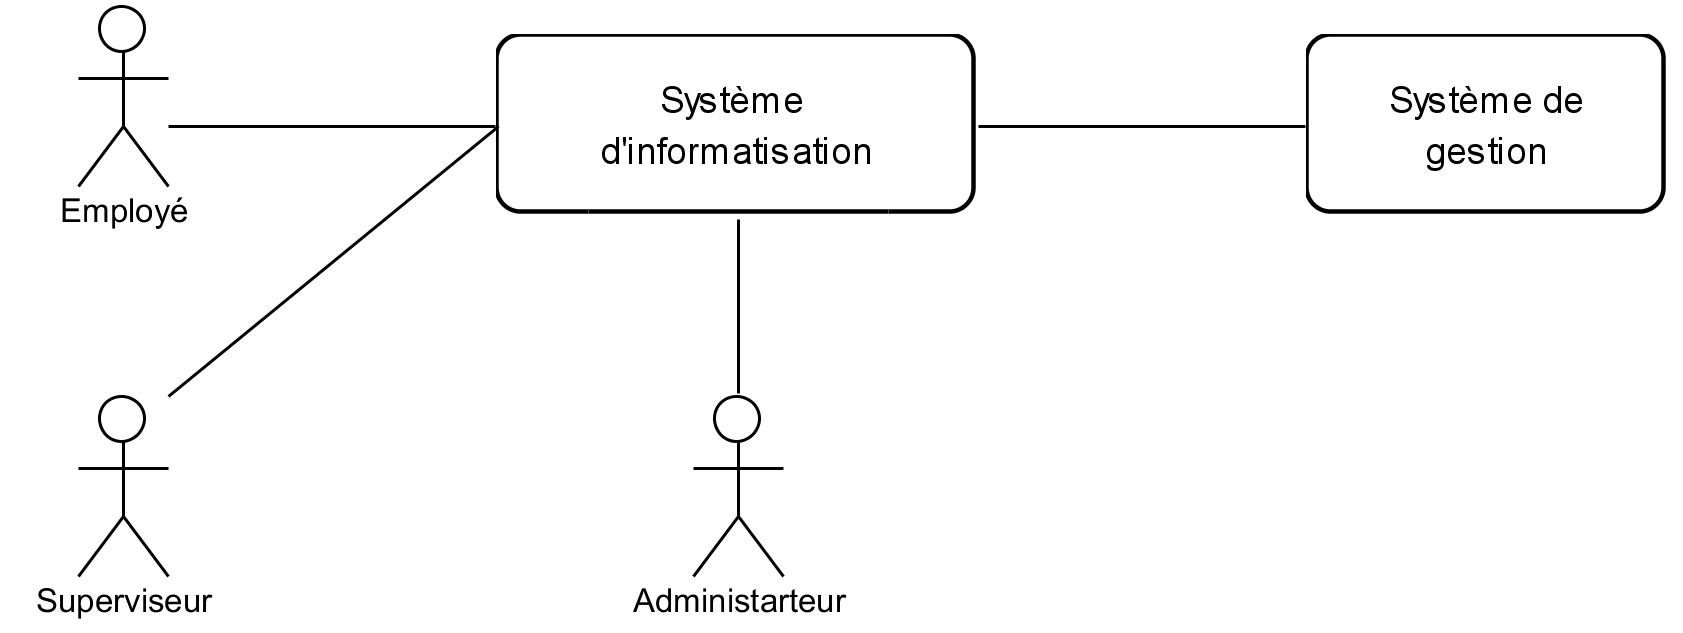
\includegraphics[scale=1.2]{images/DC}
			\caption{Diagramme de contexte du système à réaliser.}
	\end{figure}
	
	
	\clearpage
	\subsection{Identifications des cas d’utilisation}
	Le Cas d'utilisation est une description des interactions qui permettront à l'acteur d'atteindre son objectif en utilisant le système \cite{UML}. Le tableau 2.2 résume les cas d’utilisations du système à réaliser :\\
	\begin{table}[!h]
	
  	\begin{center}
	\begin{tabular}{|c|c|c|c|}
	\hline
	\textbf{N}& \multicolumn{2}{|c|}{\textbf{Cas d’utilisation}} & \textbf{Acteur}\\
	\hline
	1 & \multicolumn{2}{|c|} {S'authentifier} & \\
	\cline{1-3}
	2 & \multicolumn{2}{|c|} {Saisie des caractéristiques d'articles lors du chargement} & Employé/Superviseur\\
	\cline{1-3}
	3 & \multicolumn{2}{|c|} {Saisie des caractéristiques d'articles lors du déchargement} & \\
	\hline
	4 & \multicolumn{2}{|c|} {Gérer les employés} & Superviseur\\
	\hline
	\end{tabular}
	\caption{Cas d’utilisation du système à réaliser}
\end{center}
\end{table}
\subsection{Diagramme de cas d'utilisation}
	\begin{figure}[!h]
		\center
			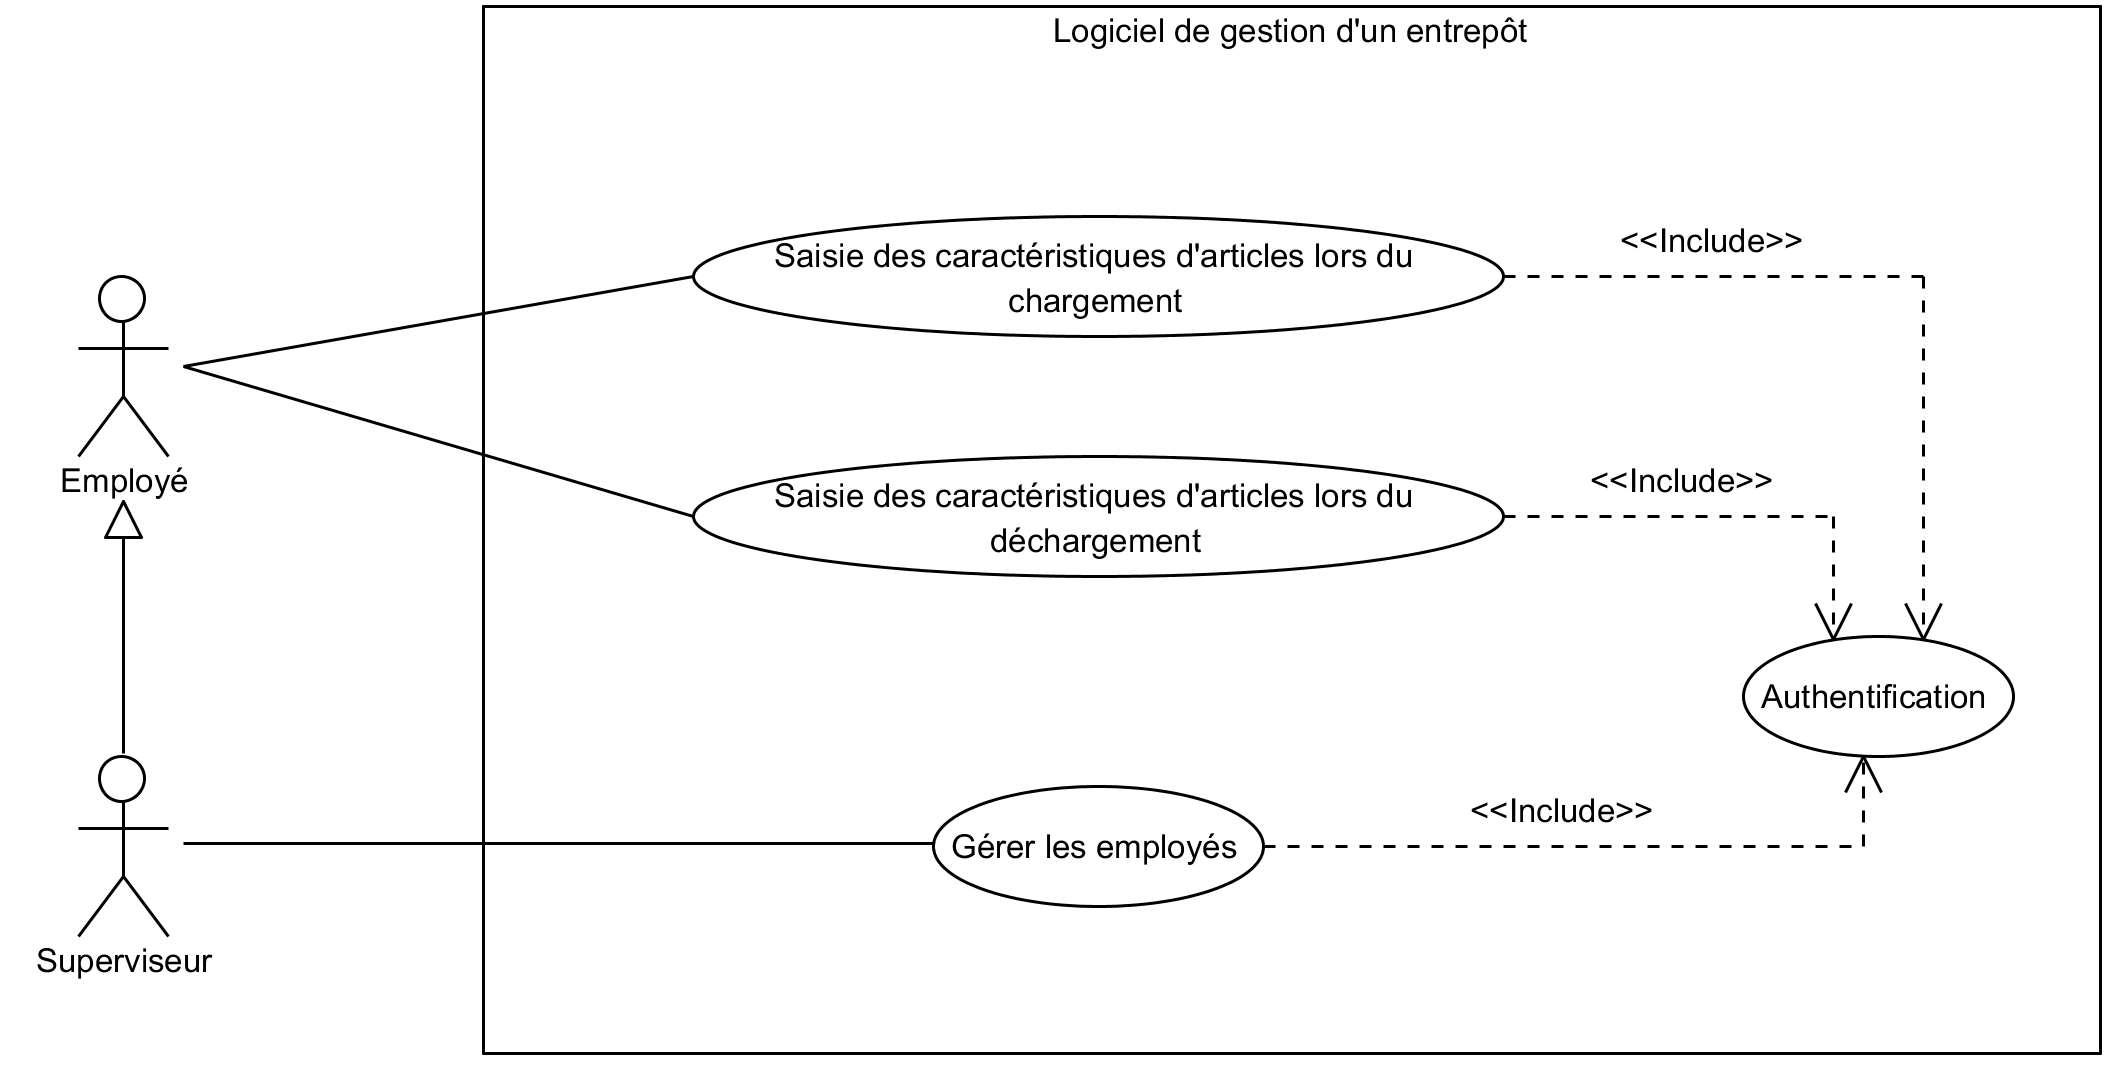
\includegraphics[scale=0.91]{images/DCD}
			\caption{Diagramme de contexte du système à réaliser.}
	\end{figure}
	\clearpage
	
	\section{Analyse des besoins}
	
\subsection{Description des cas d'utilisation}
	Les diagrammes réalisés jusqu'à maintenant (diagramme de contexte, diagramme de cas d'utilisation) nous ont permis de découvrir petit à petit les fonctionnalités que l'on devrait avoir dans le futur logiciel.
	
	Nous allons désormais parler de l'interaction entre les acteurs et le système : il s'agit de décrire la chronologie des actions qui devront être réalisées par les acteurs et par le système lui-même. Cette description va nous permettre :
	
\begin{enumerate}[label=\textbullet]
	\item clarifier le déroulement de la fonctionnalité.
	\item décrire la chronologie des actions qui devront être réalisées.
	\item d'identifier les parties redondantes pour en déduire des cas d'utilisation plus précises qui seront utilisées par inclusion, extension ou généralisation/spécialisation. Et oui, dans ce cas nous réaliserons des itérations sur les diagrammes de cas d'utilisation.
	\item d'indiquer d'éventuelles contraintes déjà connues et dont les développeurs vont devoir tenir compte lors de la réalisation du logiciel. Ces contraintes peuvent être de nature diverse.
	\end{enumerate}
	
	\subsubsection*{Cas d'utilisation <<S'authentifier>> :}
	\textbf{Cas d'utilisation} :  <S'authentifier>
	
	\textbf{Acteurs} :  <Employé,Superviseur>
	
	\textbf{Objectif} : -Il permet à l'acteur de s'authentifier.
	
	\textbf{[Pré-condition :]}  -Les identifiants de l'acteur doivent exister dans la base de donnée.
	
	\textbf{[Post-condition :]}  -Acteur Identifié	
	
	\textbf{Scénario nominal :}  1. L'acteur ouvre le logiciel.
	  
    2. Le système affiche la fenêtre d'authentification
      
    3. L'acteur saisit les identifiants
    
    4. Le système vérifie l'existence des données
     
    5. Le système identifie l'acteur.  
    \clearpage
    \textbf{Scénario alternatif :} \textit{A. Erreur d'authentification :} identifiants non valides. 
    
Cet enchaînement démarre au point 4.
   
5. Le système affiche un message d'erreur. 

Le scénario reprend au point 2.

\textbf{[Contraintes non fonctionnelles :] } <Confidentialité> 
    
    \subsubsection*{Cas d'utilisation <<Saisie des caractéristiques d'articles lors du déchargement>> :}
	\textbf{Cas d'utilisation} :  <Saisie des caractéristiques d'articles lors du déchargement>
	
	\textbf{Acteurs} :  <Employé,Superviseur>
	
	\textbf{Objectif} : - Il permet à l'acteur de 	de générer une liste où figure un emplacement 	pour 
	
	chaque article saisi.
	
	\textbf{[Pré-condition :]}  - L'article doit 	exister dans la base de donnée.
	
	\textbf{[Post-condition :]}  -Génère une 			liste où figure un emplacement pour chaque 
	
	article saisi.
	
	\textbf{Scénario nominal :} 1. L'acteur 			saisit les caractéristique de l'article.
    
    2. Le système vérifie l'existence de 				l'article.
    
     3. Le système recherche un emplacement dans 		un stock.
     
    4. Le système affiche la liste où figure un emplacement pour chaque article.  
    
    \textbf{Scénario alternatif :} \textit{A. Erreur article non-existant :} caractéristique invalide. 
    
Cet enchaînement démarre au point 2.
   
5. Le système affiche un message d'erreur. 

Le scénario reprend au point 1.

\textbf{[Contraintes non fonctionnelles :] } <Temps de réponse>


\chapter*{Conclusion}
\label{chap:Conclusion}
\addcontentsline{toc}{chapter}{Conclusion}








\end{document}